% This is samplepaper.tex, a sample chapter demonstrating the
% LLNCS macro package for Springer Computer Science proceedings;
% Version 2.20 of 2017/10/04
%
\documentclass[runningheads]{llncs}
%
\usepackage{graphicx}
% Used for displaying a sample figure. If possible, figure files should
% be included in EPS format.
%
% If you use the hyperref package, please uncomment the following line
% to display URLs in blue roman font according to Springer's eBook style:
% \renewcommand\UrlFont{\color{blue}\rmfamily}
\usepackage{cite}

\begin{document}
%
\title{A Novel Evolutionary Multi-objective Approach for Species Tree Estimation }
\author{}
\institute{}
%
\maketitle              % typeset the header of the contribution
%

\begin{abstract}
The abstract should briefly summarize the contents of the paper in
15--250 words.

\keywords{Phylogenomics  \and Multi-objective
optimization \and Evolutionary Algorithm.}
\end{abstract} 
\section{Introduction}
\label{sec:intro}
% for bioinformatics community, we don't need this introduction about phylogeny; but for evocomp, we need this
\commentM{In biological studies, evolutionary relationships between a group of organisms (usually called as taxa) are referred to as phylogeny. A hypothesis regarding such history is inferred in the form of a tree popularly known as the phylogenetic tree. A forking point in a phylogenetic tree depicts a historical speciation event which split a single population into two distinct species.  Knowledge discovered through analyzing such trees has benefited several branches if science including but not limited to medicine, forensics, bio-geography,} epidemiology~\cite{felix2015phylogenetics}. 
A species tree represents the evolutionary relationships of a group of organisms. On the other hand, the phylogeny specific to a particular region of the genome (known as locus or gene) is termed as a gene tree~\cite{maddison1997gene}. A standard approach for species tree estimation uses multiple loci, then concatenates alignments for each locus
into a super-matrix based on the assumption that all genes have the same gene tree topology~\cite{huelsenbeck1996combining, de2007supermatrix}, which is then used to estimate a species phylogeny. When all the genes evolve down the same tree topology,  sequence based statistical approaches such as maximum likelihood applied to the super-matrix are statistically consistent. 
However, gene trees may differ from each other, because genes duplicate, are lost or laterally transferred, or because alleles can coexist in populations spanning several speciation events~\cite{maddison1997gene}.
Therefore, concatenation (also known as combined analysis) can be statistically inconsistent~\cite{roch2015likelihood}, and can return incorrect trees with high confidence~\cite{kubatko-degnan-2007,edwards2007,leache-rannala,degiorgio2009}. Therefore, developing species tree estimation methods that take gene tree discordance into account has intrinsic value in phylogenomics.


%Then the super-matrix is analyzed using some sequence based statistical approaches such as maximum likelihood. However, modern studies~\cite{zwickl2014disentangling, jarvis2014whole} show that the gene trees can be discordant with each other as well as with the species tree for various biological reasons. This observation has challenges the correctness of the traditional approach and thereby motivated the researchers to develop efficient methods to estimate species tree without concatenation. 

Among the newer methods, perhaps the most popular ones belong to a family called ``summary methods''~\cite{bayzid2013naive}. They take the gene trees estimated from the individual genes as input and then find a species tree that best summarize the gene trees under various optimization criteria. 
Because incomplete lineage sorting is
expected to occur under many biologically realistic conditions (e.g., rapid radiations)~\cite{jarvis2014whole}, statistically consistent coalescent based species tree methods have been developed and are increasingly popular. 
Examples of such methods include
MP-EST~\cite{mpest}, *BEAST~\cite{heled-drummond}, NJst~\cite{njst}, BUCKy~\cite{larget-bioinf2010}, GLASS~\cite{glass}, STEM~\cite{stem}, SNAPP~\cite{snapp}, SVDquartets~\cite{svdquartet}, STEAC~\cite{steac},
ASTRAL~\cite{mirarab2014astral}, MP-EST~\cite{liu2010maximum}, NJst~\cite{liu2011estimating}, ASTRID~\cite{vachaspati2015astrid}, STELAR~\cite{islam2019stelar}, etc. Each of them optimize a particular criterion which has been shown to be statistically consistent. For an instance, ASTRAL tries to find a species tree by maximizing the number of quartets in the gene trees that are consistent with it. The quartet-score of the ASTRAL-estimated tree is expected to converge to the quartet-score of the true tree given sufficiently large numbers of true gene trees. However, with a limited number of genes and in the presence of gene tree estimation error, existing methods may \textit{overshoot} the criterion they try to optimize, and thus may deviate from the true tree. We have observed that, in most of the cases, quartet-scores of the ASTRAL trees are more than the quartet-scores of the true trees. Similarly, MP-EST, which maximizes a pseudo-likelihood measure, tends to overestimate the amount of ILS present in the gene trees~\cite{statistical-binning}. Moreover, the performance of various optimization criteria varies with varying model conditions~\cite{mirarab2014evaluating,chou2015comparative}.

Therefore, optimizing a particular optimization criterion, despite being statistically consistent, may not always produce highly accurate trees. This phenomenon motivates us to apply an evolutionary multi-objective optimization (EMO). An EMO algorithm evolves a population (i.e., a set of candidate solutions) by simultaneously optimizing multiple criteria end eventually outputs a collection of candidate solutions. 
In this study, we focus on finding a tree-space by an EMO algorithm containing highly accurate trees under practical model conditions with limited numbers of estimated gene trees. 

This is the first known study that aims to improve the accuracy of the estimated trees by multi-objective formulation. We show that if an appropriate EMO algorithm is employed to optimize different optimization criteria simultaneously, the final population is more likely to contain better species trees than the individual outputs of the existing methods. We developed an NSGA-II~\cite{deb2002fast}, a popular EMO algorithm, based framework for species tree estimation. More importantly, we designed a especially customized genetic algorithm NOSSGA (write the elaboration) whose final population contains better candidate species trees than that of the NSGA-II.  %(Section~\ref{sec:method}).
We considered three optimization criteria: quartet consistency (ASTRAL), maximum pseudo-likelihood (MP-EST), and triplet consistency (STELAR). We assessed the validity of our approach on a collection of challenging simulated dataset. Our results suggest that NOSSGA can produce a population of candidate species trees which contain substantially more accurate trees than the trees estimated by optimizing the individual criterion. \commentA{Furthermore, we explored the SPR (subtree pruning and regrafting) neighborhood of ASTRAL and MP-EST estimated trees and showed that they do not contain the highly accurate trees that can be found in the population generated by NOSSGA using multi-objective optimization.}



%To the best of our knowledge, this paper takes the first initiative to improve the accuracy of estimated species tree by existing summary methods by employing EMO algorithms.  In particular, here we makes the following key
%contributions:

\begin{comment}
\begin{itemize}
	\item We pick three optimization scores from three different methods (ASTRAL, STELAR and MP-EST) to be simultaneously optimized by an EMO algorithm (Section~\ref{sec:problem}).  
	\item We developed an NSGA-II~\cite{deb2002fast}, a popular EMO algorithm, based  framework. Also, based on obtained observations, we designed a custom genetic algorithm whose final population contains better species tree than that of the NSGA-II (Section~\ref{sec:method}). 
	\item Finally based on three simulated datasets, we examine the operation of the two EMO algorithms and then compare their performance with three existing methods (Section~\ref{sec:experiment}). 
\end{itemize}
\end{comment}


 
\section{Problem Description}
\label{sec:problem}
We are given a set of rooted binary trees as a collection gene trees each having N-taxon. We need to construct the species tree, a rooted binary tree with N-taxon, from these gene trees by simultaneously optimizing the following three objective functions:  
\begin{enumerate}[label=F\arabic*.]
		
	\item Maximize the number of consistent quartets (i.e., unrooted 4-taxon tree) between the species tree and the gene trees (used by ASTRAL\cite{mirarab2014astral})
	\item Maximize the number of consistent triplets (i.e., rooted 3-taxon tree) between the species tree and the gene trees (used by STELAR~\cite{islam2019stelar})
	\item Maximize a pseudo-likelihood estimate of the species tree utilizing the underlying triplet distribution of the gene trees (used by MP-EST~\cite{liu2010maximum})
\end{enumerate}
Each of the above functions (optimized by an existing method) has some ability to predict the species tree accuracy but none of them can necessarily lead towards the most accurate species tree. Therefore, optimizing them together, by an EMO algorithm, will generate a set of candidate solutions which is expected to contain a species tree which is more accurate than the output of the existing methods.
\section{Methodology}
\label{sec:method}
In this paper, we adapted NSGAII for species tree estimation by integrating problem-specific encoding, initialization, crossover and mutation. Moreover, we designed a special purpose EMO algorithm by modifying NSGAII considering issues associated with the problem mentioned in Section~\ref{sec:problem}. In this section, we discuss the design of our modified EMO algorithm along with its different components.


\subsection{Algorithm Design}
In general, any EMO algorithm can help to resolve issue~\ref{item:i1} by maintaining a population which contains some solutions having objectives values slightly below the domination threshold (Definition~\ref{def:domination_threshold}). But it allows optimizing one objective to a great extent even at the loss of others. Therefore, we modified NSGAII in a way that tackles issue~\ref{item:i1} more elegantly in addition to resolving issue~\ref{item:i2}.  

\begin{definition}\label{def:domination_threshold}
	\small
	We call the worst value along a particular objective in the obtained PF of a certain generation as the \textbf{domination threshold} for that objective at that generation.
\end{definition}

\begin{equation}\label{eqn:nos}
\small
NOS(x) = \sum_{i=1}^{3} \frac{F_i(x)-z_i^{min}}{z_i^{max}-z_i^{min}}
\end{equation}
{\scriptsize where $z_i^{min}$ ($z_i^{max}$) is the minimum (maximum) value of $i^{th}$ objective $F_i$ observed so far during the search process}

We replaced the non-dominated sorting by sorting based on the summation of normalized values all objective as defined by the $NOS()$ function shown in equation~\ref{eqn:nos}. That's why call the resultant algorithm as Normalized Objectives' Sum Sorting Genetic Algorithm (NOSSGA). Previously similar function was utilized in~\cite{qu2010multi}, while designing an EMO algorithm, to increase diversity and reduce computational complexity. The pseudo-code of NOSSGA in shown in Algorithm~\ref{alg:nossga}. We intensify the effect of $NOS()$ by using tournament selection based on $NOS()$ instead of the default binary tournament. We expect that selection based on $NOS()$ will discard those solutions which optimized one objective heavily at the cost of degrading others. This feature resolves issue~\ref{item:i1} more elegantly than NSGAII as well as address issue~\ref{item:i2} that NSGAII cannot handle. 

To maintain diversity of population, we always arbitrarily choose one from multiple solutions having the same $NOS()$ value (line \ref{line:diversity}). Like NSGAII, NOSSGA is a highly exploitative algorithm. To increase the exploration capability, we use crowding distance concept of NSGAII, albeit in a different way than NSGAII, to pick some least crowded solutions among the solutions with lower $NOS()$ values  (line~\ref{line:crowding_s}-\ref{line:crowding_e}). While generating offspring, we keep random selection in line~\ref{line:random_selection} to ensure the participation of such solutions. We expect that this feature will help to escape local optima.


%It optimizes three objectives, with certain attentions to the nature of the problem, and generates a tree-space that contains high quality species trees. 
%We also apply NSGAII, using the same crossover, mutation and initialization method as the NOSSGA, to approximate the PF by optimizing the three objectives. 

\begin{algorithm}[!htbp]
	\scriptsize
	\caption{NOSSGA}
	\textbf{Input:} $m_g$ (max. generations), $p_s$ (population size), $c_r$ (crossover rate), $m_r$ (mutation rate), $t_s$ (Tournament size)\\
	\textbf{Output:} $P$ (A vector of $N$ species trees)
	\begin{algorithmic}[1]\label{alg:nossga}
		\STATE{Initialize $P$ with $N$ randomly generated solutions (i.e., species trees) } \COMMENT{sec.~\ref{subsec:init}}
		\STATE{For each solution in $ P $, evaluate the objective functions and $NOS()$} \COMMENT{using eqn.\ref{eqn:nos}}
		%\STATE{For each solution $x$ in $ P $, calculate NOS($x$)}
		\STATE{$g \gets 0$} \COMMENT{generation counter}
		\WHILE{ $g < m_g$}
			\STATE{$Q \gets \emptyset$} \COMMENT{offspring population, an empty vector that can hold $N$ solutions}
			\FOR{$i \leftarrow 1$ to $p_s$}	%\label{mainLoop}	
				\STATE{$S_1 \gets$ tournament\_selection($P$, $t_s$)} \COMMENT{based on NOS()}
				\STATE{$S_2 \gets$ random\_selection($P$)} \label{line:random_selection}
				\STATE{$Q[i] \gets$ mutation(crossover($S_1, S_2, c_r$), $m_r$)} \COMMENT{sec.~\ref{subsec:crossver}, \ref{subsec:mutation}}
				%\STATE{Generate an offspring by applying crossover on $S_1, S_2$, then mutate the offspring and append the resultant solution to $Q$}		
			\ENDFOR	
			\STATE{For each solution in $ Q $, evaluate the objective functions and $NOS()$ }
			\STATE{$ R \gets P \cup Q$} \COMMENT{$R$ is a vector holding $2N$ solutions}
			%\STATE{For each solution $x$ in $ R $, calculate NOS($x$)}
			\STATE{Sort the members of $ R $ in ascending order of $NOS()$} \COMMENT{ascendind because all objectives are treated as minimization} \label{line:nos}
			\STATE{$P \gets \emptyset$, Append $R[1]$ to $P$, Remove $R[1]$ from $R$}
			%\STATE{$P[1] \gets R[1]$}
			%\STATE{$i \gets 2$}
			\FOR{$i \leftarrow 2$ to $p_s$}	%\label{mainLoop}	
				\STATE{\textbf{if} $NOS$($R[1]$) $\ne$ $NOS$(Current end of $P$), \textbf{then} Append $R[1]$ to $P$ }	\label{line:diversity}
				\STATE{Remove $R[1]$ from $R$}	\COMMENT{each element is shifted left by 1 position }
			\ENDFOR	
%			\FOR{$i \gets 1$ to $N$}	%\label{mainLoop}	
%				\IF{ NOS($R[i]) \ge P[i-1]$)}
%					\STATE{$P[i] \gets R[i]$}
%				\ENDIF
%				\STATE{Remove $R[i]$ from $R$}		
%			\ENDFOR	
			\STATE{For each remaining solution in $ R $, calculate the crowding distance}\label{line:crowding_s}
			\STATE{Sort the members of $ R $  in descending order of the crowding distance in $R$}
			\STATE{Fill-up the remaining solutions for $P$ from the top of $R$}\label{line:crowding_e}
			\STATE{$g \gets g + 1$}
		\ENDWHILE
		\STATE{\textbf{return} $P$}
	\end{algorithmic}
\end{algorithm}

\subsection{Crossover}\label{subsec:crossver}
We used Prune-Delete-Graft (PDG)~\cite{villalobos2018memetic} as the crossover operator which generates one tree (i.e., offspring) from two parents. At first, It takes a random sub-tree from
one of the parents. Then it inserts the selected sub-tree in the other parent at a
randomly selected insertion point. Finally it deletes duplicated species
from the second tree and returns it as the output.

\subsection{Mutation} \label{subsec:mutation}
Our mutation operator applies one of the three widely used tree rearrangement strategies~\cite{felsenstein2004inferring}: (i) Nearest Neighbour
Interchange (NNI), (ii) Sub-tree Pruning and Re-grafting
(SPR) and (iii) Tree Bisection and Reconnection (TBR). Each of them is selected randomly with equal probability. NNI
exchanges sub-trees from an arbitrary internal branch to obtain
a new tree. SPR picks a random sub-tree from a tree, removes it and then re-grafts it in a random
position to generate a new tree. TBR combines both
SPR and NNI.

\subsection{Solution Initialization}\label{subsec:init}
We utilized the given set of gene trees initializing the population. We randomly pair two gene trees and apply our crossover operator on them to generate an initial solution


\subsection{Implementation Notes}
We encoded species tree using \textit{TreeTemplate} class provided by BIO++~\cite{gueguen2013bpp} which is a collection of C++ libraries for Bioinformatics. We implemented both NSGAII and NOSSGA using jMetalCpp\footnote{\url{https://github.com/jMetal/jMetalCpp}} which is a C++ framework for EMO. We used the implementation of PDG, NNI, SPR and TBR from~\cite{zambrano2016mo} after fixing several bugs. We evaluated each objective (QT/TP/PL) using a feature provided by each method (ASTRAL/STELAR/MP-EST) to score an existing species tree. Thus for each candidate solution, we invoked the executable of a particular method to evaluate an objective.

\begin{comment}
\subsection{Objective Evaluation}
Each method (ASTRAL, STELAR or MP-EST) provides an option to score an existing species tree. We used this feature enable to evaluate the objectives. Thus for each candidate species tree, we invoke the executable of a particular method (ASTRAL/STELAR/MP-EST) to evaluate an objective . %We converted each objective into minimization to conform 
%We evaluated each objective by executing the method that 
%: invoke java executable
%MP-EST: Maximize branch length, c++ executable
\end{comment}
\section{Experimental Studies}
\label{sec:experiment}
We examine the difference in operation of NSGAII and NOSSGA and evaluate their performance with respect to three existing methods (ASTRAL, MP-EST and STELAR) based on three simulated datasets: 10-taxon (\#estimated gene tree: 200)~\cite{bayzid2015weighted}, 11-taxon (\#estimated gene tree: 50)~\cite{chung2011comparing} and 15-taxon (\#estimated gene tree: 100)~\cite{statistical-binning}. Each of them has 10 replicates (R1 to R10). We used False Negative (FN) rate~\cite{bayzid2013naive} to measure the accuracy of the estimated species tree. FN rate expresses the fraction of edges present in the true species tree but missing in the estimated tree. %previously studied

\begin{figure}
	\begin{adjustwidth}{-4cm}{-3cm}
		\centering	
		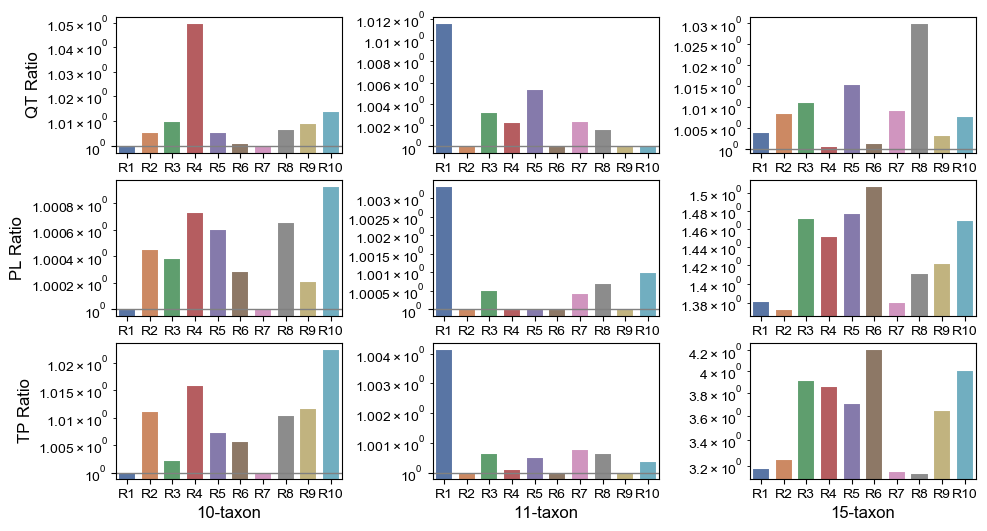
\includegraphics[width=1.6\textwidth]{Figure/tool_ratio}
		\caption{The issue of overshooting the optimization criterion beyond the true tree by existing methods. Each row shows the ratio of scores (QT/PL/TP), optimized by a particular method (ASTRAL/MP-EST/STELAR), of the true tree to that of the estimated tree by the same method.} \label{fig:tool_ratio}
	\end{adjustwidth}

\end{figure}

\subsection{Observation}
\label{subsec:observation}
At first, we present an important observation that essentially motivated us to tackle the problem of species tree estimation as a MOP. We mentioned in Section~\ref{sec:intro} that, due to limitation in available knowledge, existing methods may overshoot the criterion they try to optimize, and thus may deviate from the true tree. In Fig.~\ref{fig:tool_ratio}, we summarize our observations for three methods (ASTRAL, MP-EST and STELAR) on 10 replicates of our selected datasets. Here, the top row shows the ratio of quartet-scores (QT) of the true trees to quartet-scores (QT) of the ASTRAL-estimated trees. Likewise, the middle row shows the pseudo-likelihood (PL) ratio of the true trees and MP-EST estimated trees and the bottom row does the same with triplet (TP) ratio of STELAR. As we treat each objective as a minimization form, ideally these ratios should be 1 (marked as gray horizontal line in each plot). However, we find that in most of the cases the ratio is greater than 1. %And for 15-taxon (third column of Fig.~\ref{fig:tool_ratio}), we 


\subsection{NSGAII vs. NOSSGA}
Here we thoroughly inspect the behavioral difference between NSGAII and NOSSGA to know whether NOSSGA posses our desired properties. To ensure a level playing field, we ran both algorithms with the same configuration (independent run: 15 , population size: 100, maximum evaluations: 10000, crossover rate: 0.3, mutation rate: 1.0). For NOSSGA, we use tournament size 10.


\subsubsection{Correlation between two objectives:} We show the variation of correlation between each pair of objectives with generations for NSGAII and NOSSGA on three datasets in Fig.~\ref{fig:gen_wise_correlation}. The plotted correlation coefficients are averaged over 15 runs and 10 replicates. We see that, contrary to NSGAII, NOSSGA is able to avoid conflict between any two objectives along the whole period according to our expectation\footnote{Nayeem link it to the method section in algo}. 

\begin{figure}[!htbp]
	%\scriptsize
	\centering
	\begin{adjustwidth}{-1cm}{-1cm}
		\begin{subfigure}[b]{0.4\textwidth}
			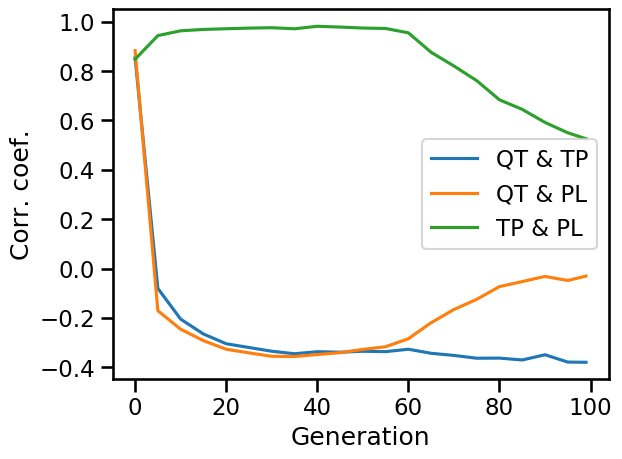
\includegraphics[width=\textwidth]{Figure/10-taxon_NSGAII_corr_plot}
			\caption{NSGAII: 10-taxon}
			%\label{fig:con_pr06}
		\end{subfigure}%
		\begin{subfigure}[b]{0.4\textwidth}
			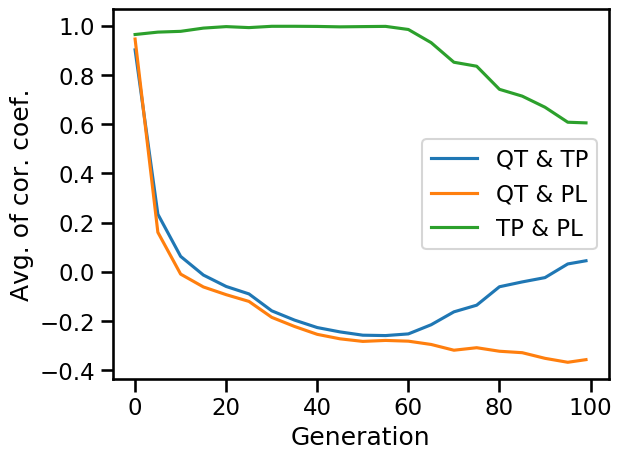
\includegraphics[width=\textwidth]{Figure/11-taxon_NSGAII_corr_plot}
			\caption{NSGAII: 11-taxon}
			%\label{fig:con_pr07}
		\end{subfigure}%
		\begin{subfigure}[b]{0.4\textwidth}
			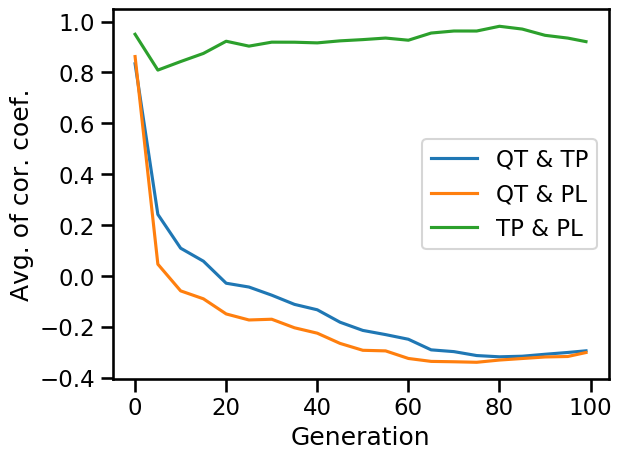
\includegraphics[width=\textwidth]{Figure/15-taxon_NSGAII_corr_plot}
			\caption{NSGAII: 15-taxon}
			%\label{fig:con_pr09}
		\end{subfigure}	
		\begin{subfigure}[b]{0.4\textwidth}
			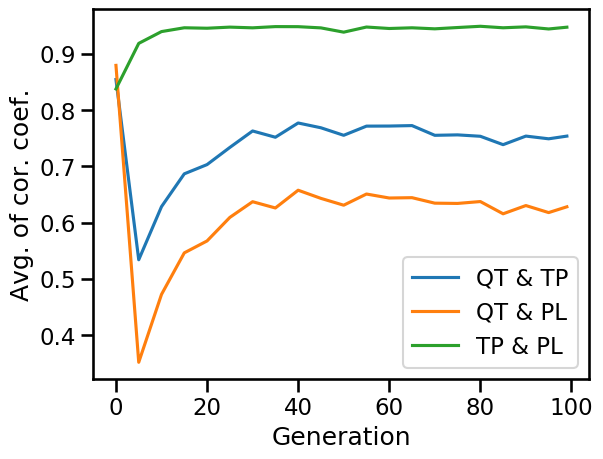
\includegraphics[width=\textwidth]{Figure/10-taxon_NOSSGA_corr_plot}
			\caption{NOSSGA: 10-taxon}
			%\label{fig:con_pr06}
		\end{subfigure}%
		\begin{subfigure}[b]{0.4\textwidth}
			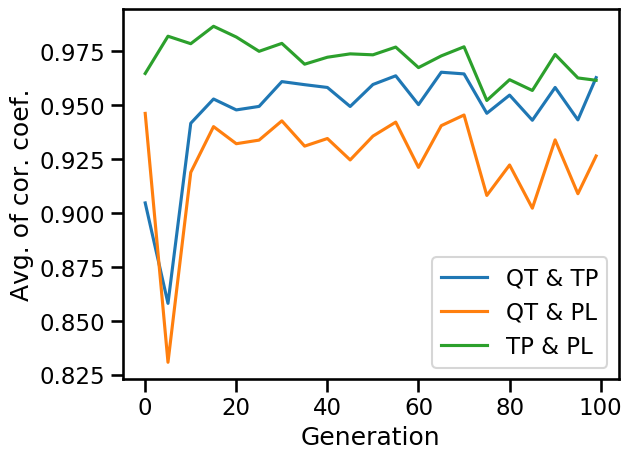
\includegraphics[width=\textwidth]{Figure/11-taxon_NOSSGA_corr_plot}
			\caption{NOSSGA: 11-taxon}
			%\label{fig:con_pr07}
		\end{subfigure}%
		\begin{subfigure}[b]{0.4\textwidth}
			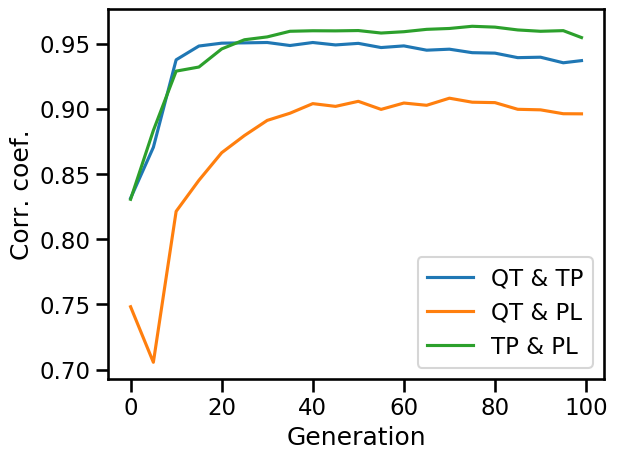
\includegraphics[width=\textwidth]{Figure/15-taxon_NOSSGA_corr_plot}
			\caption{NOSSGA: 15-taxon}
			%\label{fig:con_pr09}
		\end{subfigure}
		\caption{Variation of correlation between each pair of objectives with generations for NSGAII and NOSSGA on three datasets. 
			%The plotted correlation coefficients are averaged over 15 runs and 10 replicates. 
			%In each plot (algorithm: dataset), the correlation coefficient of each point are averaged over 15 runs and 10 replicates.
		}
		\label{fig:gen_wise_correlation}
	\end{adjustwidth}
\end{figure}

\subsubsection{Diversity of objectives and FN rate:}\label{subsubsec:diversity} Fig.~\ref{fig:gen_wise_std_dev} shows the variation of standard deviation of three objectives and FN rates\footnote{The knowledge of FN rate is absent to the EMOs.} in the population with generations for NSGAII and NOSSGA on three datasets. In each plot, the standard deviation values are averaged over 15 runs and 10 replicates. This figures establish that NSGAII loses diversity at early stages possibly due to discarding dominated solutions.    
\begin{figure}[!htbp]
	\centering
	\begin{adjustwidth}{-1cm}{-1cm}
		\begin{subfigure}[b]{0.4\textwidth}
			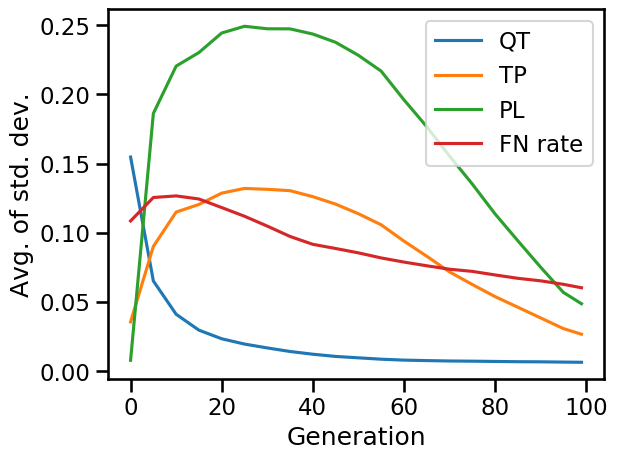
\includegraphics[width=\textwidth]{Figure/10-taxon_NSGAII_std_dev}
			\caption{NSGAII: 10-taxon}
			%\label{fig:con_pr06}
		\end{subfigure}%
		\begin{subfigure}[b]{0.4\textwidth}
			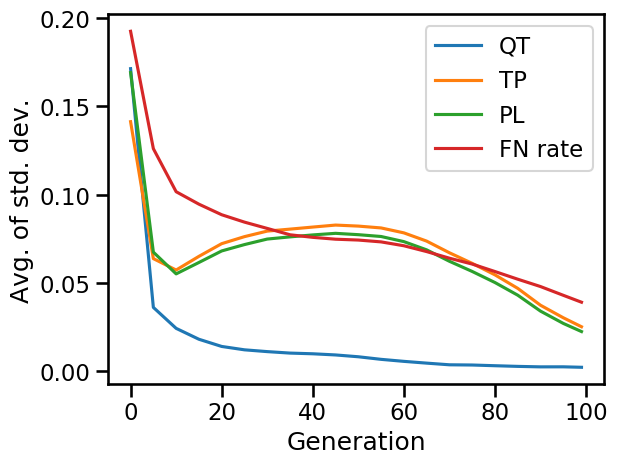
\includegraphics[width=\textwidth]{Figure/11-taxon_NSGAII_std_dev}
			\caption{NSGAII: 11-taxon}
			%\label{fig:con_pr07}
		\end{subfigure}%
		\begin{subfigure}[b]{0.4\textwidth}
			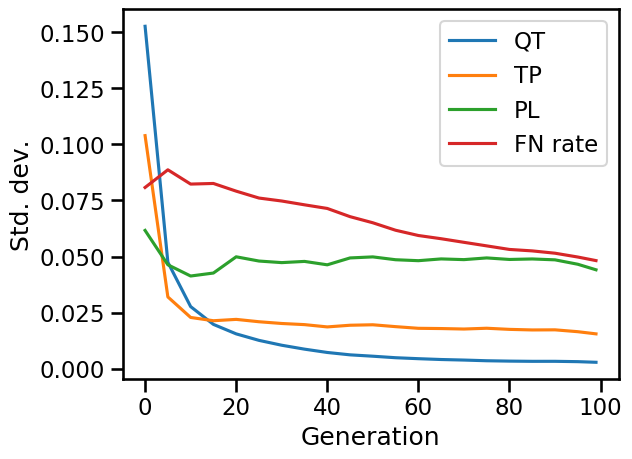
\includegraphics[width=\textwidth]{Figure/15-taxon_NSGAII_std_dev}
			\caption{NSGAII: 15-taxon}
			%\label{fig:con_pr09}
		\end{subfigure}
		\begin{subfigure}[b]{0.4\textwidth}
			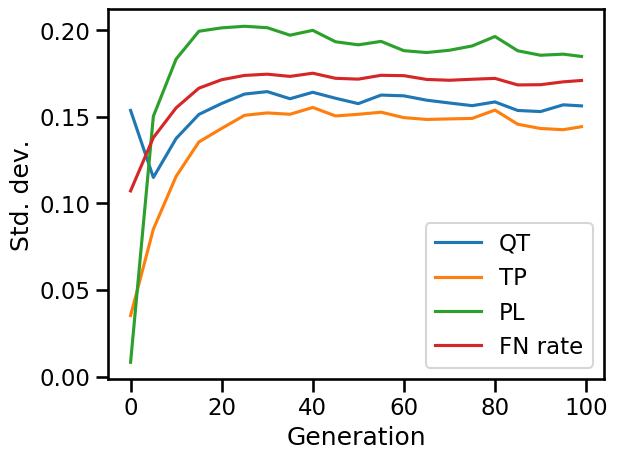
\includegraphics[width=\textwidth]{Figure/10-taxon_NOSSGA_std_dev}
			\caption{NOSSGA: 10-taxon}
			%\label{fig:con_pr06}
		\end{subfigure}%
		\begin{subfigure}[b]{0.4\textwidth}
			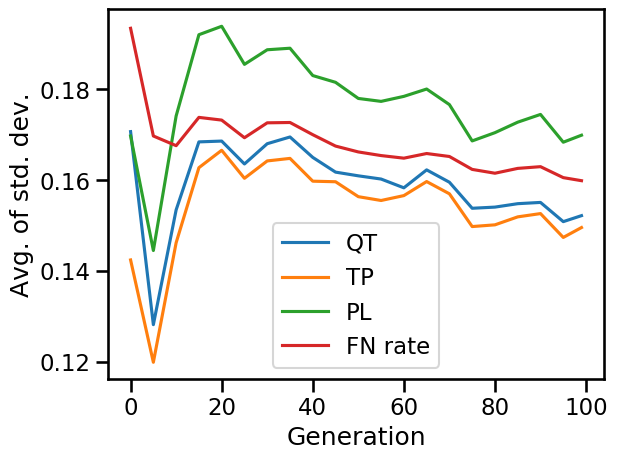
\includegraphics[width=\textwidth]{Figure/11-taxon_NOSSGA_std_dev}
			\caption{NOSSGA: 11-taxon}
			%\label{fig:con_pr07}
		\end{subfigure}%
		\begin{subfigure}[b]{0.4\textwidth}
			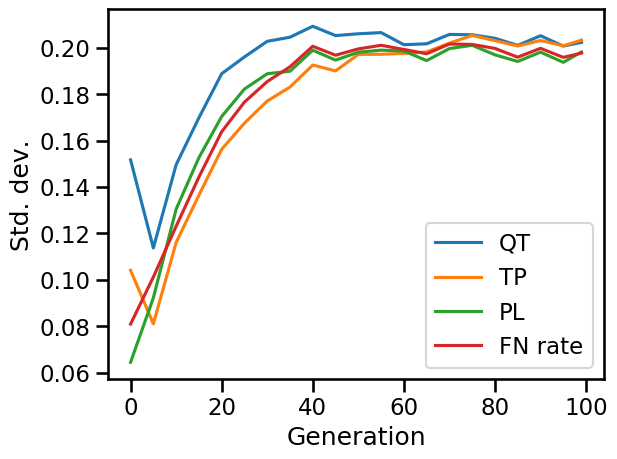
\includegraphics[width=\textwidth]{Figure/15-taxon_NOSSGA_std_dev}
			\caption{NOSSGA: 15-taxon}
			%\label{fig:con_pr09}
		\end{subfigure}
		\caption{Variation of standard deviation of three objectives and FN rates in the population with generations for NSGAII and NOSSGA on three datasets.
			% on three datasets. The plotted standard deviations are averaged over 15 runs and 10 replicates. 
		}
		\label{fig:gen_wise_std_dev}
	\end{adjustwidth}
\end{figure}

\subsubsection{Improvement in objectives and FN rate:} Now we observe how the best (minimum) value of three objectives\footnote{we treated each objective as a minimization} and FN rate\footnote{lower is better} in the population improves across generations for NSGAII and NOSSGA as depicted in Fig.~\ref{fig:gen_wise_min}. The plotted minimum values are averaged over 15 runs and 10 replicates. NSGAII allows the objectives (except PL\footnote{To decrease the large runtime of PL calculation using MP-EST, we decreased the default iteration count}) to improve as much as possible which causes the resultant species tree to deviate from the true tree. As a result, the best FN rate of NSGAII starts to degrade after a particular generation. On the other hand, to avoid such deviation, NOSGGA restrict the objectives to improve after a certain point in time. So its FN rate continues to improve.
\begin{figure}[!htbp]
	\centering
	\begin{adjustwidth}{-1cm}{-1cm}
		\begin{subfigure}[b]{0.4\textwidth}
			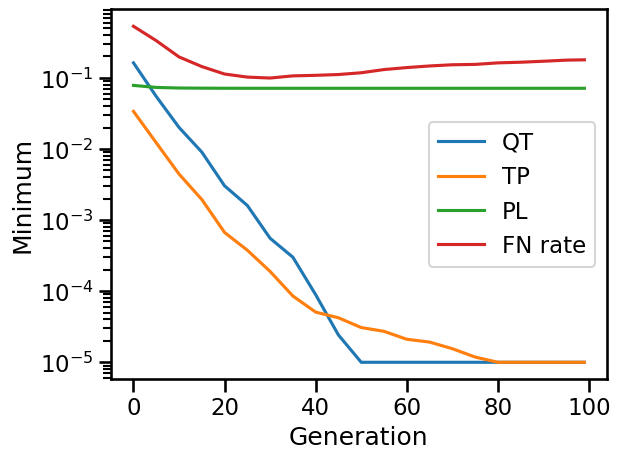
\includegraphics[width=\textwidth]{Figure/10-taxon_NSGAII_minimum}
			\caption{NSGAII: 10-taxon}
			%\label{fig:con_pr06}
		\end{subfigure}%
		\begin{subfigure}[b]{0.4\textwidth}
			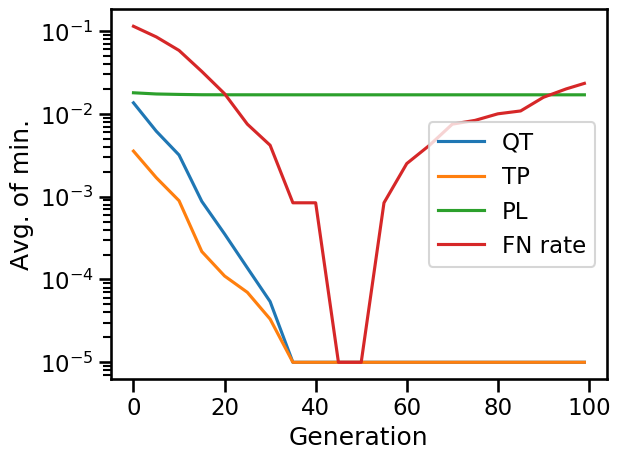
\includegraphics[width=\textwidth]{Figure/11-taxon_NSGAII_minimum}
			\caption{NSGAII: 11-taxon}
			%\label{fig:con_pr07}
		\end{subfigure}%
		\begin{subfigure}[b]{0.4\textwidth}
			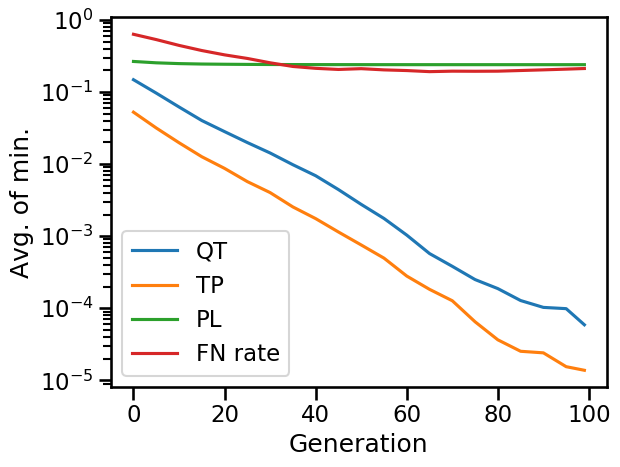
\includegraphics[width=\textwidth]{Figure/15-taxon_NSGAII_minimum}
			\caption{NSGAII: 15-taxon}
			%\label{fig:con_pr09}
		\end{subfigure}
		\begin{subfigure}[b]{0.4\textwidth}
			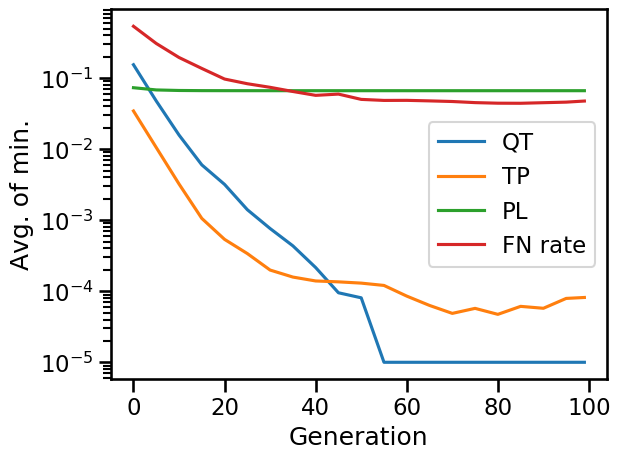
\includegraphics[width=\textwidth]{Figure/10-taxon_NOSSGA_minimum}
			\caption{NOSSGA: 10-taxon}
			%\label{fig:con_pr06}
		\end{subfigure}%
		\begin{subfigure}[b]{0.4\textwidth}
			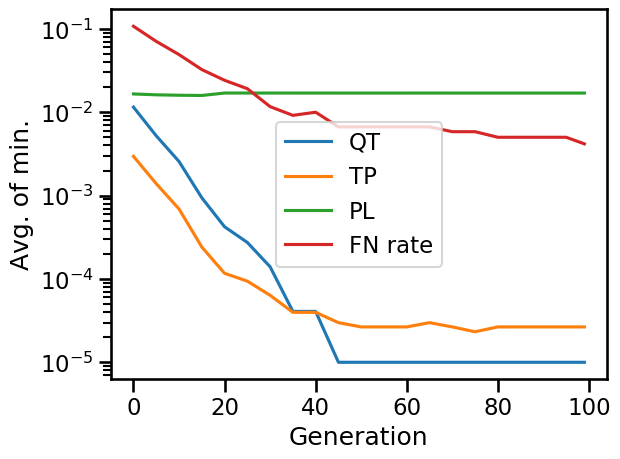
\includegraphics[width=\textwidth]{Figure/11-taxon_NOSSGA_minimum}
			\caption{NOSSGA: 11-taxon}
			%\label{fig:con_pr07}
		\end{subfigure}%
		\begin{subfigure}[b]{0.4\textwidth}
			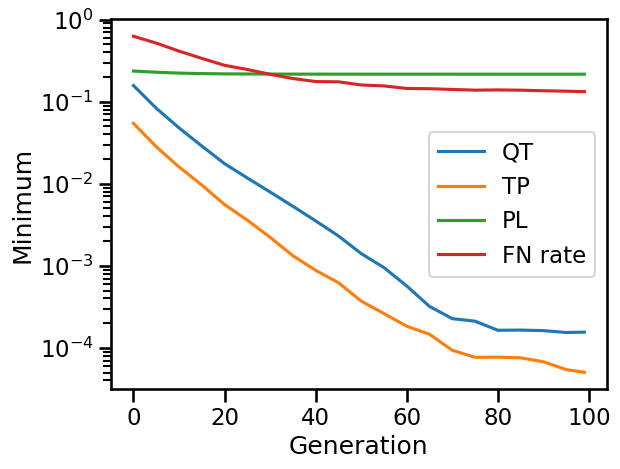
\includegraphics[width=\textwidth]{Figure/15-taxon_NOSSGA_minimum}
			\caption{NOSSGA: 15-taxon}
			%\label{fig:con_pr09}
		\end{subfigure}
		\caption{Variation of minimum of three objectives and FN rates in the population with generations for NSGAII and NOSSGA on three datasets.
			%The plotted minimum values are averaged over 15 runs and 10 replicates. 
		}
		\label{fig:gen_wise_min}
	\end{adjustwidth}
\end{figure}

\subsubsection{Comparison based on hypervolume:} We mentioned earlier that for the problem that we deal in this paper is different than the traditional MOPs. Importantly, the definition of convergence for MOPs is not applicable for our problem. To explore this issue, we compare NSGAII and NOSSGA in terms of hypervolume (HV)~\cite{zitzler1999multiobjective} which is probably the most popular measure to evaluate the performance of an EMO. HV captures both convergence and diversity in a single real-value. For MOPs with all minimization objectives, a higher value of HV is desirable. In Fig.~\ref{fig:gen_wise_hv}, we plot the HV values averaged over 15 runs and 10 replicates. From these results, it is difficult to differentiate between these two algorithms. Both of their HV values get saturated at early generation. Interestingly, according to HV, NOSSGA seems better than NSGAII. This is probably due to the loss of diversity at an early stage as we saw earlier. 
\begin{figure}[!htbp]
	\centering
	\begin{adjustwidth}{-1cm}{-1cm}
		\begin{subfigure}[b]{0.4\textwidth}
			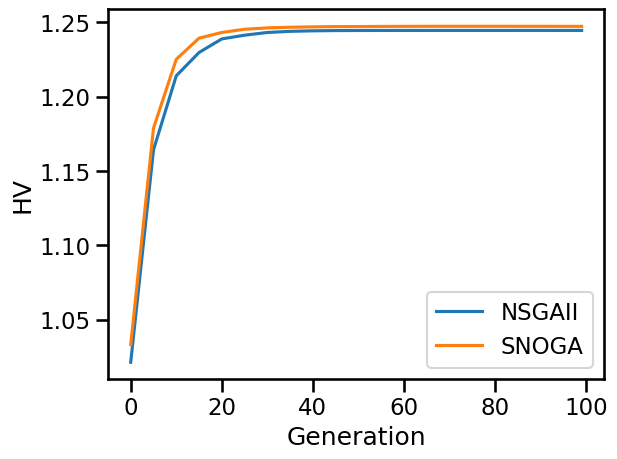
\includegraphics[width=\textwidth]{Figure/10-taxon_hv}
			\caption{10-taxon}
			%\label{fig:con_pr06}
		\end{subfigure}%
		\begin{subfigure}[b]{0.4\textwidth}
			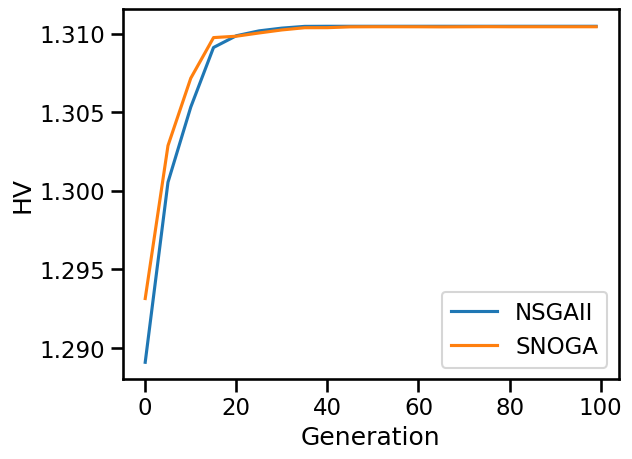
\includegraphics[width=\textwidth]{Figure/11-taxon_hv}
			\caption{11-taxon}
			%\label{fig:con_pr07}
		\end{subfigure}%
		\begin{subfigure}[b]{0.4\textwidth}
			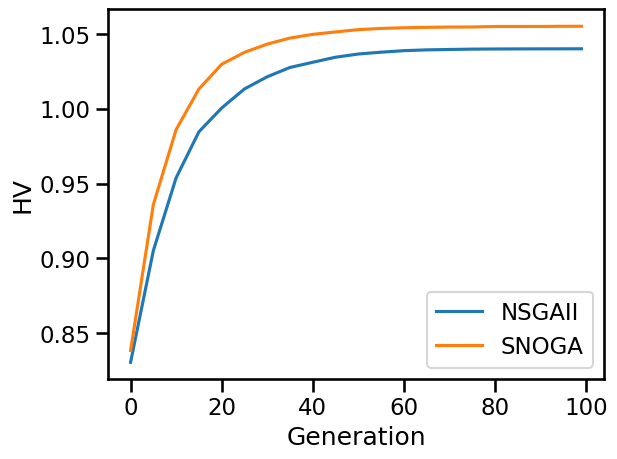
\includegraphics[width=\textwidth]{Figure/15-taxon_hv}
			\caption{15-taxon}
			%\label{fig:con_pr09}
		\end{subfigure}
		\caption{Variation of HV with generations for NSGAII and NOSSGA on three datasets.}
		\label{fig:gen_wise_hv}
	\end{adjustwidth}
\end{figure}
\subsubsection{Tree accuracy:} Finally we compare NSGAII and NOSGGA in terms of the tree accuracy for 10 replicates of each dataset. So we graphically summarize the FN rate (a lower value means more accurate) of the best trees from the final population of 15 independent runs using boxplots in Fig.~\ref{fig:emo_compare}. We observe that, NOSSGA can offer much better solutions than NSGAII in almost all cases. In some cases, the two algorithm perform equally.
\begin{figure}
	\centering
	\begin{adjustwidth}{-2cm}{-2cm}
		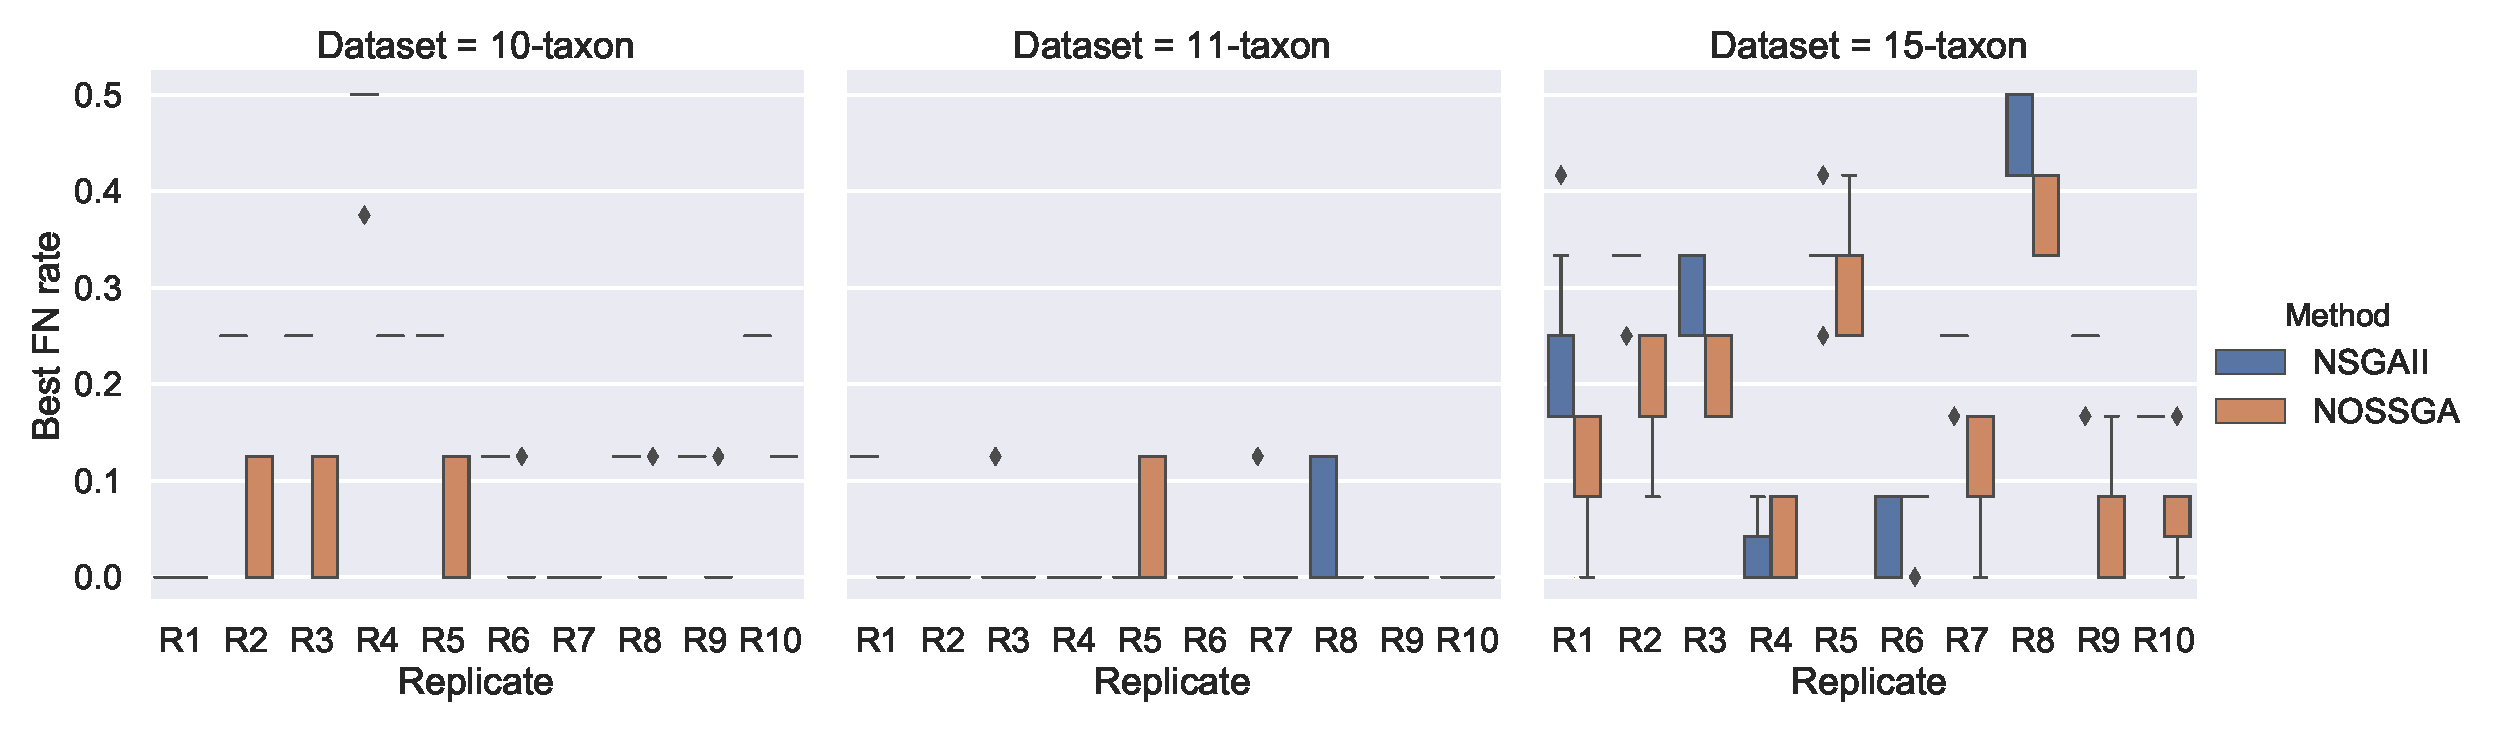
\includegraphics[width=1.5\textwidth]{Figure/emo_boxplot}
		\caption{Accuracy of the best estimated species trees extracted from the final population of NSGAII and NOSSGA on each dataset having 10 replicate.} \label{fig:emo_compare}
	\end{adjustwidth}
\end{figure}

\begin{figure}
	\begin{adjustwidth}{0cm}{0cm}
		\centering
		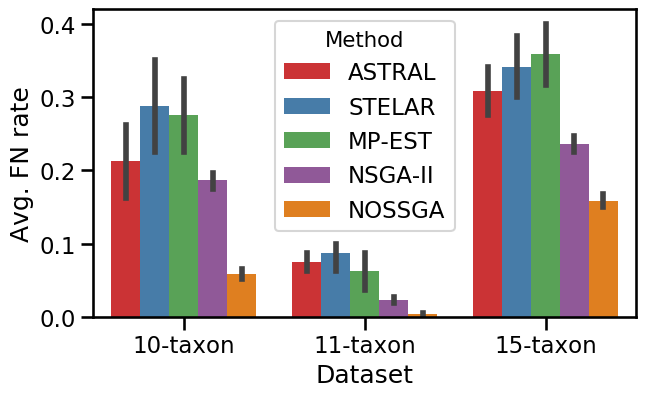
\includegraphics[width=0.8\textwidth]{Figure/all_dataset_compare}
		\caption{Performance comparison of ASTRAL, STELAR, MP-EST, NSGAII and NOSSGA on three datasets. 
			%We show the average FN rates with standard error bars over 10 replicates
		} \label{fig:compare_exisitng_methods}
	\end{adjustwidth}
\end{figure}

\subsection{Comparison with Existing Methods}
We evaluated the best trees offered by NSGAII and NOSSGA in comparison with the output of ASTRAL, MP-EST and STELAR. ASTRAL and MP-EST are two of the most widely used and accurate
summary methods. We ran the exact version of ASTRAL and STELAR, which are guaranteed to return the globally optimal tree. And for MP-EST, we ran with 10 random starting points and selected the species tree with the
highest PL value. For each dataset, we show the average FN rates with standard error bars over 10 replicates in Fig.~\ref{fig:compare_exisitng_methods}. We find that NOSSGA offers the most accuracy. In all datasets, the accuracy of NOSSGA is at least 2X than ASTRAL. Even the basic NSGAII is more accurate than all of the three existing methods. These results clearly demonstrate the benefit of treating this problem as a MOP. 


%\subsection{Discussion}

\begin{comment}
\begin{figure}[!htbp]
	\centering
	\begin{adjustwidth}{-1cm}{}
	\begin{subfigure}[b]{0.55\textwidth}
		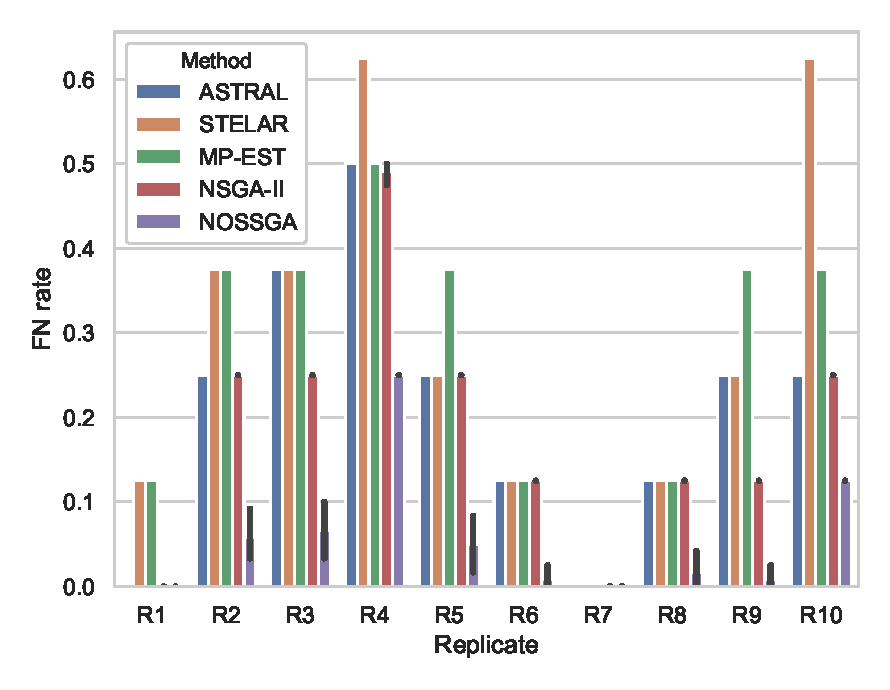
\includegraphics[width=\textwidth]{Figure/10-taxon_10_replicates}
		\caption{10-taxon}
		%\label{fig:con_pr06}
	\end{subfigure}%
	\begin{subfigure}[b]{0.55\textwidth}
		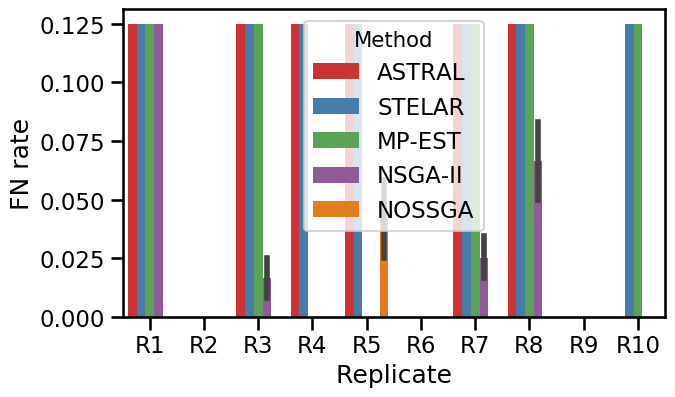
\includegraphics[width=\textwidth]{Figure/11-taxon_10_replicates}
		\caption{11-taxon}
		%\label{fig:con_pr07}
	\end{subfigure}%
%	\newline

	\begin{subfigure}[b]{0.55\textwidth}
		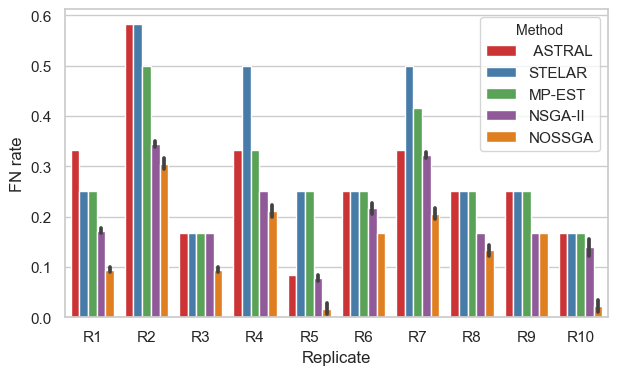
\includegraphics[width=\textwidth]{Figure/15-taxon_10_replicates}
		\caption{15-taxon}
		%\label{fig:con_pr09}
	\end{subfigure}
	\begin{subfigure}[b]{0.55\textwidth}
		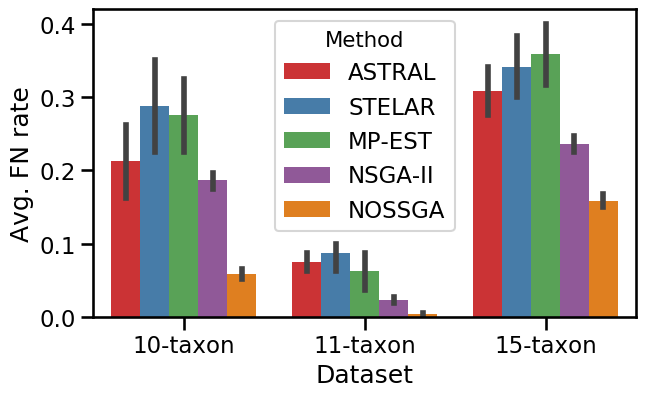
\includegraphics[width=\textwidth]{Figure/all_dataset_compare}
		\caption{Summary}
		%\label{fig:con_pr09}
	\end{subfigure}%

	\caption{Comparison of ASTRAL, STELAR, MP-EST, NSGAII and NOSSGA on 10 replicates of 3 datasets.}
	\label{fig:datasets}
\end{adjustwidth}
\end{figure}



\begin{figure}[!htbp]
\centering
\begin{adjustwidth}{-1cm}{}
\begin{subfigure}[b]{0.48\textwidth}
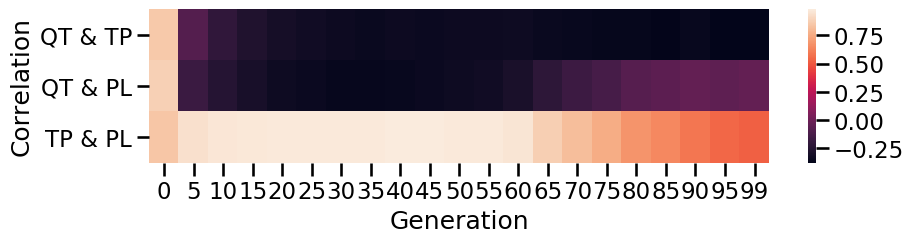
\includegraphics[width=\textwidth]{Figure/10-taxon_NSGA-II_heatmap}
\caption{NSGAII: 10-taxon}
%\label{fig:con_pr06}
\end{subfigure}%
\begin{subfigure}[b]{0.4\textwidth}
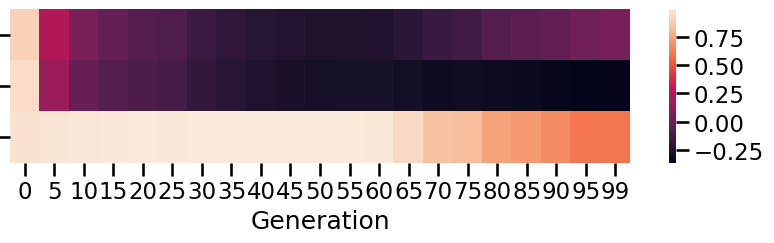
\includegraphics[width=\textwidth]{Figure/11-taxon_NSGA-II_heatmap}
\caption{NSGAII: 11-taxon}
%\label{fig:con_pr07}
\end{subfigure}%
\begin{subfigure}[b]{0.4\textwidth}
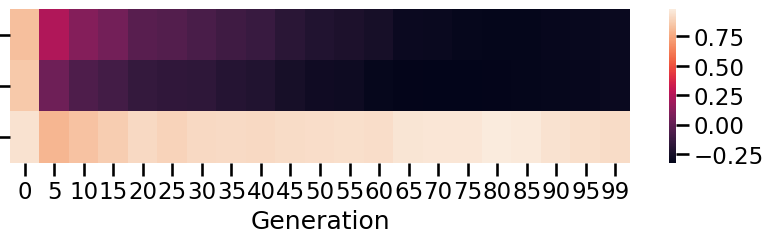
\includegraphics[width=\textwidth]{Figure/15-taxon_NSGA-II_heatmap}
\caption{NSGAII: 15-taxon}
%\label{fig:con_pr09}
\end{subfigure}

\begin{subfigure}[b]{0.48\textwidth}
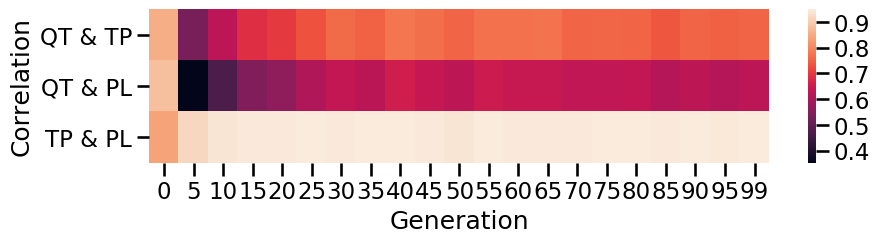
\includegraphics[width=\textwidth]{Figure/10-taxon_NOSSGA_heatmap}
\caption{NOSSGA: 10-taxon}
%\label{fig:con_pr06}
\end{subfigure}%
\begin{subfigure}[b]{0.4\textwidth}
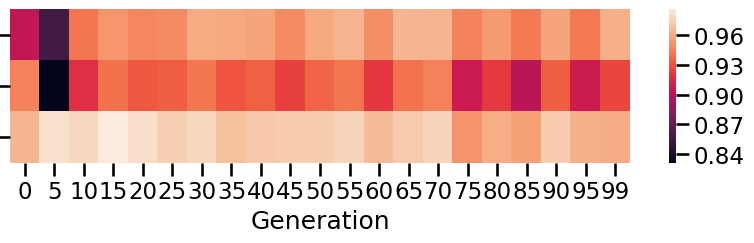
\includegraphics[width=\textwidth]{Figure/11-taxon_NOSSGA_heatmap}
\caption{NOSSGA: 11-taxon}
%\label{fig:con_pr07}
\end{subfigure}%
\begin{subfigure}[b]{0.4\textwidth}
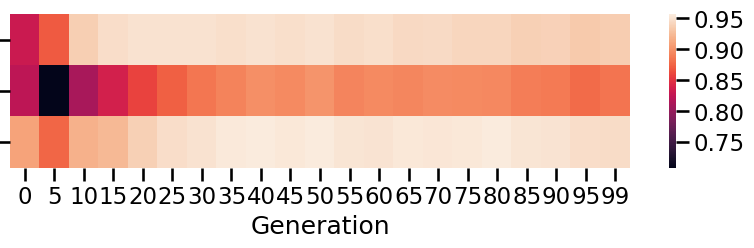
\includegraphics[width=\textwidth]{Figure/15-taxon_NOSSGA_heatmap}
\caption{NOSSGA: 15-taxon}
%\label{fig:con_pr09}
\end{subfigure}
\caption{Correlation between each pair of objectives as the generation of an EMO progresses. For each dataset, we average the correlation coefficient over 15 runs and 10 replicates.}
\label{fig:gen_wise_correlation}
\end{adjustwidth}
\end{figure}
%\begin{figure}
%	\centering
%	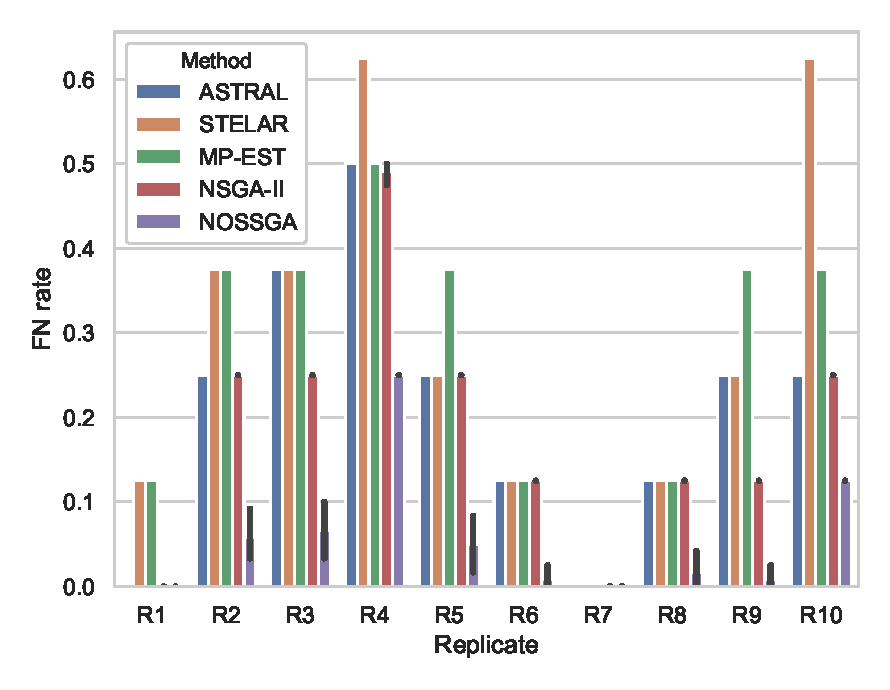
\includegraphics[width=0.6\textwidth]{Figure/10-taxon_10_replicates}
%	\caption{10-taxon.} \label{fig1}
%\end{figure}
%\begin{figure}
%	\centering
%	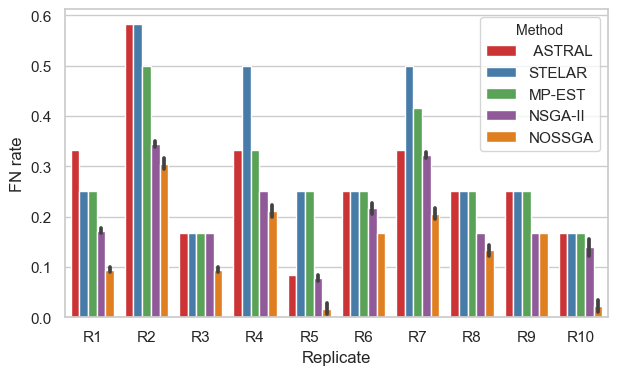
\includegraphics[width=0.6\textwidth]{Figure/15-taxon_10_replicates}
%	\caption{15-taxon.} \label{fig2}
%\end{figure}
\subsection{Results on 10-taxon dataset}
\subsection{Results on 11-taxon dataset}
\subsection{Results on 15-taxon dataset}
\end{comment}


\section{Conclusion and Future Work}
In this paper we introduced the problem of estimating species tree from a set of gene trees as a MOP. We showed with examples that the existing method, optimizing a single criterion, may overshoot the criterion and thus deviate from the true species tree. We selected three objectives from three existing methods. Unlike traditional MOPs, in this problem a dominated solution is often important than a non-dominated one and hence we cannot rely on the PF to contain highly accurate trees. Therefore, we designed a specialized EMO algorithm, namely, NOSSGA, which is a simplification of NSGAII. NOSSGA is able to generate a tree-space containing highly accurate trees. We analyzed the difference of behavior between NOSSGA and NSGAII. Finally, we found the accuracy of the best trees offered by NOSSGA is quite better three existing methods on a collection of challenging simulated dataset. 

We are currently working to devise a systematic methodology to filter a limited number of better trees from the final population without the knowledge of true tree provided with the simulated dataset. At present, out mutation selects one from NNI/SPR/TBR at random with equal probability. We will improve it by adjusting the selection probabilities in an adaptive way based on the success rate of an operator in the previous generation. Also, we are planning make NNI/SPR/TBR behaving intelligently by utilizing the common patterns found across the gene trees. To enable NOSSGA processing large datasets within a reasonable time, we are improving the efficiency of objective evaluations. Moreover, we are modifying another popular EMO algorithm, namely, MOEA/D, in a way to make it effective to tacke this problem.


%
% ---- Bibliography ----
%
% BibTeX users should specify bibliography style 'splncs04'.
% References will then be sorted and formatted in the correct style.
%
\bibliographystyle{splncs04}
\bibliography{main_bib}
\end{document}
